\documentclass[english,a4paper,babel,12pt]{nitathesis}

%%%%%%%%%%%%%%%%%%%%%%%%%%%%%%%%%%%%%%%%%%%%%

\usepackage{graphicx,times,epsfig,amsmath}
%\usepackage[Sonny]{myfancy}
\usepackage[Sonny]{fncychap}
\usepackage{float}
\usepackage{xspace}
\usepackage{algorithmwh}
\usepackage{comment}
\usepackage{watermark}
\usepackage{graphicx}
\usepackage{pifont}
\usepackage{fancyhdr}
\usepackage{blindtext}
%\usepackage{lscape}
\usepackage{rotating}
\usepackage{ragged2e}
\usepackage{comment}
\usepackage{nomencl}
\numberwithin{figure}{chapter}
\usepackage{placeins}
%\usepackage{sectsty}

%%%%%%%%%%%%%%%%%%%%%%%%%%

%%%%%%%%%%%%%%%%%%%%%%%%%%
\lhead{}
\chead{}
%\rhead{CSED, NIT Agartala}
\lfoot{ }
\cfoot{\thepage}
\rfoot{}
%\setlength{\headrulewidth}{0.4pt}
%\setlength{\footrulewidth}{0.4pt}

\renewcommand{\headrulewidth}{0.5pt}
\renewcommand{\footrulewidth}{0.5pt}
%%%%%%%%%%%%%%%%%%%%%%%%%%



%\usepackage{algorithms}% \Add{} and \Del{} Corrections and \Mark{}
\begin{document}

% Using the watermark package which is in StyleFiles/
% and to remove DRAFT COPY ONLY appearing on the top of all pages comment out below line
%\watermark{SAMPLE COPY ONLY}



\beforepreface
\prefacesection{Acknowledgement}
We would like to take this opportunity to express our deep sense of gratitude to all who helped us directly or indirectly
 during this thesis work.\\
Firstly, we would like to thank our supervisor, \textbf{Mr. Supervisor Name}, for being a great mentor and the best adviser 
we could ever have. Her advise, encouragement and critics are source of innovative ideas, inspiration and causes behind the successful completion of this report. The confidence shown on us  by her was the biggest source of inspiration for us. It has been a privilege working with her from last one year.\\
We are highly obliged to all the faculty members of Computer Science and Engineering Department for their support and encouragement. We also thank  \textbf{Prof.(Dr.)~Gopal~Mugeraya}, Director, NIT Agartala and \textbf {Mr. Mrinal Kanti Deb Barma}, H.O.D, CSED for providing excellent computing and other facilities without which this work could not achieve its quality goal.\\


\begin{comment}
 Finally, I am grateful to my \textbf{parents} for their support. It was impossible for me to complete 
this thesis work without their love, blessing  and
encouragement.
\end{comment}

\vspace*{0.5cm} 
\hspace*{1cm}\textbf{\large - Candidate's Name}
\hspace*{6cm}\textbf{\large - Candidate's Name}

\vspace*{0.5cm} 
\hspace*{1cm}\textbf{\large - Candidate's Name}
\hspace*{6cm}\textbf{\large - Candidate's Name}
 
%\vspace*{0.5cm} \hspace*{1cm}\textbf{\large - Candidate's Name}

\pagestyle{fancy}
\fancyhead[RO,RE]{\nouppercase\rightmark}
\fancyfoot[C]{\thepage}
\listoffigures
\listoftables
\newpage
\prefacesection{Abstract}
\blindtext





% COMMENTED BY RAJIB \prefacesection{Abstract}
% COMMENTED BY RAJIB \justifying

% COMMENTED BY RAJIB \blindtext




%\afterpreface
%\pagenumbering{roman}                     
%\setcounter{page}{12}
\renewcommand{\headrulewidth}{0.5pt}
\pagestyle{fancy}
\fancyhead[RO,RE]{\nouppercase\rightmark}
\fancyfoot[C]{\thepage}
%\fancyhead[RO,RE]{\thepage}
\tableofcontents
\newpage



% This 13 is for total page before chapters starts
%COMMENTED BY RAJIB \listoffigures
%COMMENTED BY RAJIB \listoftables
%\pagenumbering{roman}
%\setcounter{page}{11}
\newpage
\pagenumbering{arabic}
\setcounter{page}{1}   

\fancyhf{}
\fancyhead[RO]{\slshape\nouppercase\rightmark{}}
\fancyhead[RE]{\slshape\nouppercase\leftmark{}}
\cfoot{\thepage}
\pagestyle{fancy}
%\fancyhead[ro]{\slshape\nouppercase\thepage}
%\fancyhead[re]{\slshape\nouppercase\thepage}
%\fancyhead[ro,re]{\slshape\nouppercase\thepage}

\flushbottom

\chapter{Introduction}
 
   \blindtext

\section{Motivation}
 \blindtext
\section{Goal}
 \blindtext   
\section{Contribution of the Dessertation}
 \blindtext
 
 \begin{table}
 \begin{center}
 \caption{First Sample Table}
 \begin{tabular}{|c|c|}
 \hline
 B.Tech & CSE\\
 \hline
 M.Tech & ECE\\
 \hline
 Ph.D & EIE\\
 \hline 
 \end{tabular}
 \end{center}
\end{table}  
  

 

\flushbottom

\flushbottom
\chapter{Related Work}
\section{IEEE Learning Technology System Architecture (LTSA)}
The IEEE 1484 learning technology standard committee (LTSC) developed an system architecture specification for learning technology. 
It is known as Learning Technology System Architecture (LTSA).\par
  An architecture specification, LTSA, is being developed in close collaboration with the Aviation Industry CBT Committee (AICC),
the European Commission PROmoting Multimedia access to Education and Training in EUropean Society
(PROMETEUS) initiative (EC/DGXIII), the European Union Projects Allianceof Remote Instructional Authoring and Distribution Networks 
for Europe (ARIADNE), the European CEN/ISSS Workshop European Committee for Standardization, Information Society Standardization 
System, Learning Technologies Workshop (CEN/ISSS/LT) on learning technology and the IMS Project and Advanced
Distributed Learning (ADL). The LTSA proposes the top level architecture for system design. LTSA model is generic enough to get applied on a variety of learning systems from different domains. LTSA covers a 
wide range of learning technology, computer-based training, electronic performance support systems, computer assisted instruction, 
intelligent tutoring, education and training technology, metadata, etc\cite{ltsa}.
\subsection{IEEE LTSA Architecture Description}
The five different levels of the architecture represent the different points of view of
a learning process\cite{ltsa} (figure.1)
\begin{itemize}
 \item \textit{Layer 1}: This level defines the tasks of acquisition, transfer, exchange and
discovery for the learner as a result of the interactions with his environment. The
level is seen as two systems exchanging information.
 \item \textit{Layer 2}: This layer defines the learner’s reaction to the environment. The
definition is based on the specific design features of learner related modules.
  \item \textit{Layer 3}: A component system, normalized by IEEE, defines an organization
of a learning process, seen from the data and control flow point of view.
  \item \textit{Layer 4}: This level exploits the component system, directly, in order to
formalize the technological design constraints. It allows the identification of the
system’s activities during the learning process. This provides the genric views of
all the stakeholders and therefore, takes care of their interest.
  \item \textit{Layer 5}:  \blindtext
\end{itemize}
\begin{comment}
\begin{figure}[htb]
 \centering
 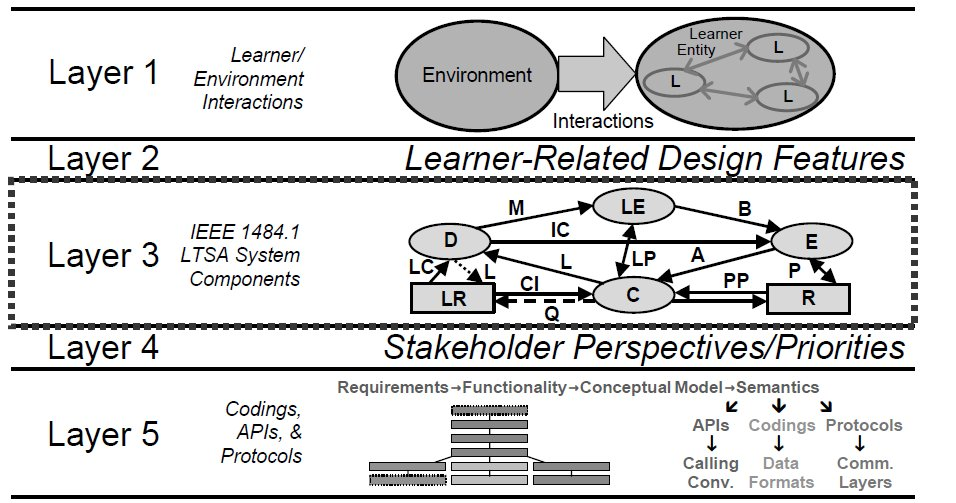
\includegraphics[scale=.4]{m.jpg}
 % m.jpg: 956x503 pixel, 72dpi, 33.73x17.74 cm, bb=0 0 956 503
 \caption{IEEE LTSA Layered Structure\cite{ltsa}}
\end{figure}
\end{comment}
\subsection{A detailed description of LTSA system components at level 3}
 \blindtext types used are \cite{ltsa} (figure.2):
\begin{enumerate}
 \item \textit{The interaction context:} This flow of data gives the necessary information for
    interpretation of the observations.
\item \textit{The observations:} This represents the real-time unabridged information concerning the learner activities.
\item \textit{The acquisition state:} The evaluating process can send or update a learner profile (e.g. a response to a correct answer within a given time).
\item \textit{The learner profile:} The tutoring process can consult and modify learner information during the apprenticeship. This is a data-store
    which updates the learner profile as per data-base management system dictat.
\item \textit{The evaluation:} It informs the tutoring process of the present state of the
    learner profile so as to optimize the learning process.
\begin{comment}
\begin{figure}[htb]
 \centering
 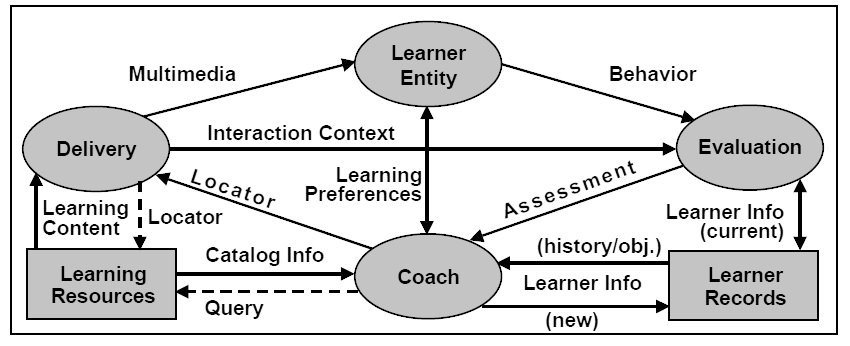
\includegraphics[scale=.6]{rj.jpg}
 % rj.jpg: 850x346 pixel, 72dpi, 29.99x12.21 cm, bb=0 0 850 346
 \caption{IEEE LTSA Layer-3 (System Components)\cite{ltsa}}
\end{figure}
\end{comment}
\item  \textit{The learner preferences:} The tutoring process negotiates the teaching parameters with the learning actor(s).
\item  \textit{The multimedia data:} This flow of data allows the learning process to use simultaneous pedagogical multimedia resources such as video, audio, text and
    graphics. All these contents are devloped and designed as per scheme of e-Learning.
\item  \textit{The locality:} This data or control flow indicates where to find a given pedagogical resource.
\item  \textit{The pedagogical contents:} This data flow has the coded pedagogical material. The content presentation, in an appropriate format, is an
    outcome of this data flow.
\item  \textit{The catalogued inquiries and information:} The tutoring process can carry out
    simple requests to find appropriate learning objects for a course. These requests
    may contain search criteria based on the learner’s preferences, the evaluation
    results and the course information.

\end{enumerate}
   The role and the behavior of the different components are described using a
learner scenario, which is divided into eight identified scenarios:
\begin{enumerate}
 \item The teaching style, the pedagogical choices and the acquisition methods are
negotiated with the learner.
\item The learning process is observed and evaluated in a context of action and
interaction with the system.
\item The evaluating process gives observations and indications about the learner
style and/or information about the functioning /the state of the system.
\item This data is stored in a data bank dedicated to the learner.
\item The tutoring process analyses the learner’s performance from his assessments,
his preferences, his past history and his future perspectives.
\item This same process searches for suitable learning object using resource bank
requests.
\item The tutoring process extracts the pedagogical content from the proposed
resources. It transmits the resource references to the diffusion process, organizing
them, for example, into a pedagogical sequence.
\item The diffusion process extracts the pedagogical contents from the learning
object to adapt it to the surrounding interface used by the learner.

\end{enumerate}

\subsection{Limitations of LTSA for e-Learning services}
Some of the functional areas, that is not included in LTSA, are identified :
\begin{itemize}
 \item The model does not regard the learning object designer as an integrated
component in the learning process.
 \item The students evaluation records are stored but, the use is not specified. This
brings ambiguity in case of e-Learning services to be provided and e-Learning services to be received to give services. 
The composition of services becomes difficult.
 \item For a distance mode learner, if the learner possesses some wrong/incomplete
idea at the start and the feedback system fails to identify it, then the LTSA layer
2 algorithm falls apart under a never ending iterative cycle. The learner can never
be sure, that his learning activities are properly registered. Moreover, the system
never recognizes the incomplete feedback or shows the partial data that may have
been registered for the future use.
 \item Students counseling is not included in the LTSA architecture. Students enrol
courses by only knowing the name of the course without knowing the prerequisites
or eligibility. Being in different service mode, these components are scheduled to
run with one another and most of the time behaves like stand-alone service module.
The selection of the courses is left to student’s rationale and intuition without a
suggestion from the mentor. The lack of student counselling makes the e-Learning
system weaker than a formal education system.
 \item The model is based on client server, component based system. There is
still possibility of making LTSA component more reuseable, loosely coupled and
increasing the modularity of LTSA by extending it into SOA environment. The
component may be used as services. But mapping the components into services
does not fit into typical Client-Server architecture.

 
\end{itemize}




\section{Mapping IEEE LTSA Framework in Client Server Model}
 \blindtext
\begin{figure}[htb]
 \centering
 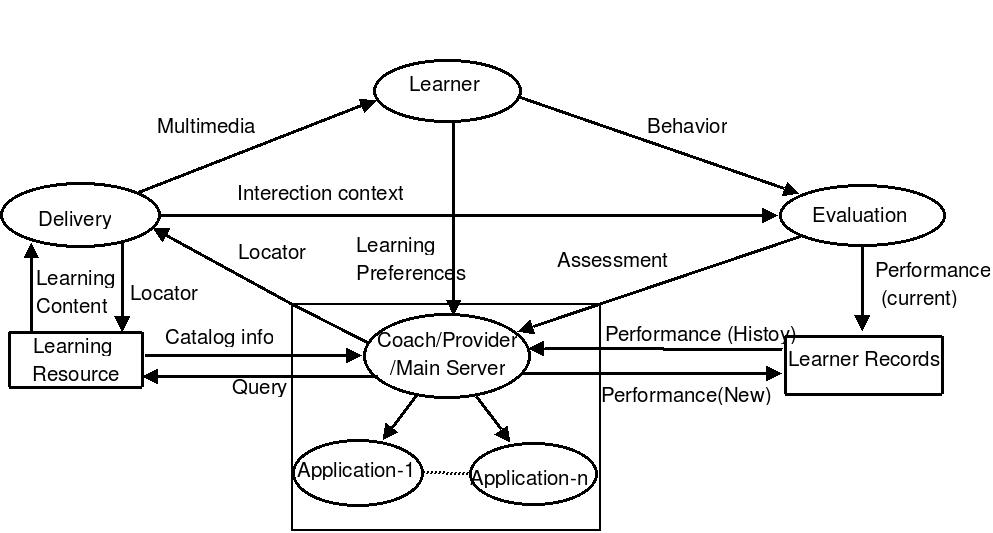
\includegraphics[scale=.5]{IeeeLtsa.jpeg}
 % IeeeLtsa.jpeg: 993x533 pixel, 72dpi, 35.03x18.80 cm, bb=0 0 993 533
 \caption{IEEE LTSA Client Server Architecture\cite{ltsa}}
\end{figure}

\subsection{Limitation of client-server based IEEE LTSA framework}
IEEE LTSA client server architecture is suitable for utilizing stand alone service
components as evident from figure. 3 These service components do not own any responsibility towards offering themselves for preparation of composite services. It is
obvious that composition compatability of services only comes as an after thought
in this architecture making it as a ’limited service’ architecture. Other limitations
are:
\begin{itemize}
 \item  Learning content provider (server) may not be able to resolve concurrency.
Many learner might try to connect to server at the same time. As any learner may
like to connect at any time, it creates a bottleneck due to lack of concurrency. Even
it may lead to typical denial of services (DoS).
 \item Since the learner and provider component may be devloped by different vendors, they may not be compatible with respect to data type, language, platform
etc.
 \item Replication of provider due to different customization may make data inconsistant.
 \item It is incapable of providing real time services and therefore, works in a limited
way in interactive mode. The security remains limited to authentication of the
learner. Multilevel security is usually not employed. The architecture generally
works in trust based security mode. It heavily relies on operating system security
features e.g. in unix OS, frequent use of 'chmod' command.
\end{itemize}
\section{Security Framework}
 \blindtext C\&C module \cite{cc}.

\section{Mapping IEEE LTSA Framework in Proposed Distributed System Architecture For Improvement}
In a distributed system, learner actively issue requests to objects in servers. Servers
passively provide access to objects that respond to client requests. Clients and
servers are usually at different address spaces. Clients and servers both may be
located on several machines physically (Figure.4). 
\begin{figure}[h!]
 \centering
 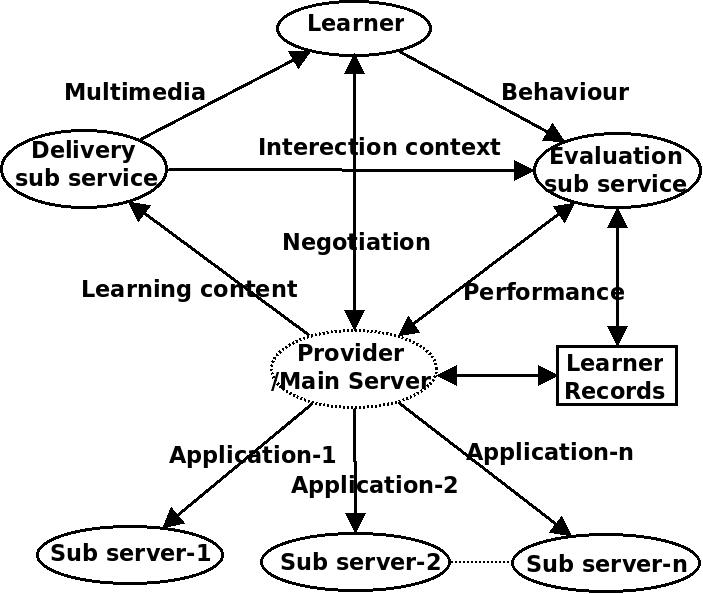
\includegraphics[scale=.5]{ds2.jpeg}
 % ds2.jpg: 961x831 pixel, 100dpi, 24.41x21.11 cm, bb=0 0 692 598
 \caption{IEEE LTSA in Distributed System Architecture}
\end{figure}

\subsection{Capabilities in the DSA for e-Learning}
Distributed system broadens the scope of service composition by implementing
compatability of services. Other capabilities of the system for e-Learning framework
are as follows:
\begin{itemize}
 \item This open system architecture allows new learning resources to be added to
it, as and when required.
 \item System is flexible and scalable.
 \item It is possible to reconfigure the system dynamically.
  \item No need to decide on locations for learning applications, each application can
work at any location.
 \item No need of providing service compatibility separately, if a standard is followed.
\item Concurrency of proccesses can be ensured by the very design of the architecutre.

\end{itemize}



\subsection{Limitation of the Architecture}
\begin{itemize}
 \item Systems are very complicated to design and implement.
\item Incapable of providing composite services unless predefined through a standard
 technology.
\item System is not as much scalable as it should be in case of e-Learning requirement
 to cater the need of different learners of different capabilities and requirements.

\end{itemize}

\subsection{Security for the proposed Distributed e-learning System}
Security remains to be closely linked with performance of a e-Learning system in
a distributed environment. While considering security from LTSA point of view,
the design elements must take care of information access control, various security
handlers and other security related processing (e.g. Kerboros or any other third
party authentication server) \cite{fox}.
\subsubsection{Information Access and Control}  \blindtext
 \subsubsection{ Security Handlers/ Processing} \blindtext
minimally considered and must be the focus of active research for preparing secured
service composition in e-Learning system \cite{car}.

\subsection{Security Challenges for the extending e-Learning services}
 \blindtext  as \cite{car}:
\begin{itemize}
 \item  \blindtext
 \item Network attacks usually target specific applications. The adaptation of control and coordination among the different mechanisms, whose capabilities are used
in the adaptive response, is needed.
\end{itemize}
 \blindtext

\flushbottom

\flushbottom
\chapter{Mapping of IEEE LTSA Framework in Service Oriented Architecture (SOA) for further Improvement}
 \blindtext, as was
the case with the components \cite{lan}.
\begin{figure}[h!]
 \centering
 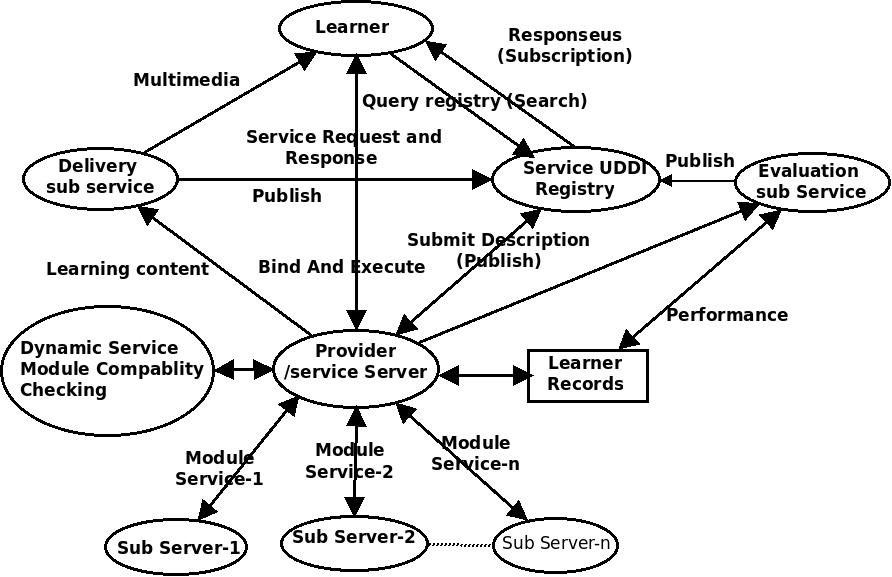
\includegraphics[scale=.5]{s0ajournal.jpeg}
 % s0ajournal.jpeg: 892x577 pixel, 72dpi, 31.47x20.36 cm, bb=0 0 892 577
 \caption{IEEE LTSA in SOA environment}
\end{figure}

    \blindtext.\\

   The proposed extended model of IEEE LTSA makes use of SOA architecture
(Figure. 5). \blindtext
\section{Capabilities of the proposed Service Oriented Architecture based IEEE LTSA Model}
The analysis of the model as presented in Figure. 5 brings out the following inherent
capabilities in the proposed extended model of IEEE LTSA:
\begin{itemize}
 \item \textit{Reusability}- SOA based IEEE LTSA model provide reuseability of learning services because they are loosly coupled. A new composition of different services
is possible by permutation, combination of the services and feasibility of their composition.
\item \textit{Interoperability}- SOA based model stresses interoperability, the ability of
systems using different platforms and languages to communicate with each other.
Each learning service provides an interface that can be invoked through a connector
type. An interoperable connector consists of a protocol and a data format, that
each of the potential user of the service understands. Interoperability is achieved
by supporting the protocol and data formats of the service’s current and potential
users including learners.
\item \textit{Loose Coupling}- Coupling refers to the number of dependencies between
modules. There are two types of coupling: loose and tight. Loosely coupled modules have a few well-known dependencies. Tightly coupled modules have many well
known as well as unknown dependencies. Every software architecture strives to
achieve loose coupling between modules. SOA promotes loose coupling between
service consumers and service providers. A few well-known dependencies between
consumers and providers may even be restored to become independent under imposed conditions. This may promote the composed components
 or modules to perform efficiently without infection of other components and modules. The conditional loose coupling allows to run 
the composed service faster in a stand alone
manner.
\item \textit{Flexibility}-The loosely-coupled, document-based, asynchronous nature of
services in an SOA allows e-learning applications to be flexible. With changing
requirements, the adaptability comes faster.
\item \textit{Capability of providing composite e-learning services}- The proposed framework is having the capability like scaling, 
suitability of high performance, customerization and coupling/decoupling of services depending upon the circumstances.

\end{itemize}


\flushbottom

\flushbottom
\chapter{Validation of Proposed Models: Case Study-IGNOU web portal}
\section{Description of IGNOU Flexilearn System}
\Blindtext
 with following features:
\begin{itemize}
 \item Any visitor to FlexiLearn site has the option to register for any particular
course or a full length academic programme. A modular approach is followed
wherein a registered learner can combine course credit to obtain a deploma or
degree of his/her own choice.
\item The platform provides self learning environment with a list of academic advisors/course guide to act as mentors.The personal learning environment will have
interactive tools like discussion board, wikis, podcasting, RSS feeds etc.
\item Each course will have the opton for both online assessment as well as offline
one, as per the choice of learner. Examination is conducted ’on demand’.
 \item A complete mechanism is integrated through the e-portfolios of individual
learners. e-portfolio keep a formal record of all formal and informal studies carried
out by the registered learner. Certification of the course will be based on the
stipulated time spent on a course and completion of all learning activities identified
by the faculty for the fulfilment of the course requirement. It may have formal
elements like any other education system e.g. grades, evaluation, rechecking etc.

\end{itemize}
\section{Mapping of Flexilearn System into IEEE LTSA in SOA}
\blindtext
 services in Figure. 7.


\begin{figure}[htb]
 \centering
 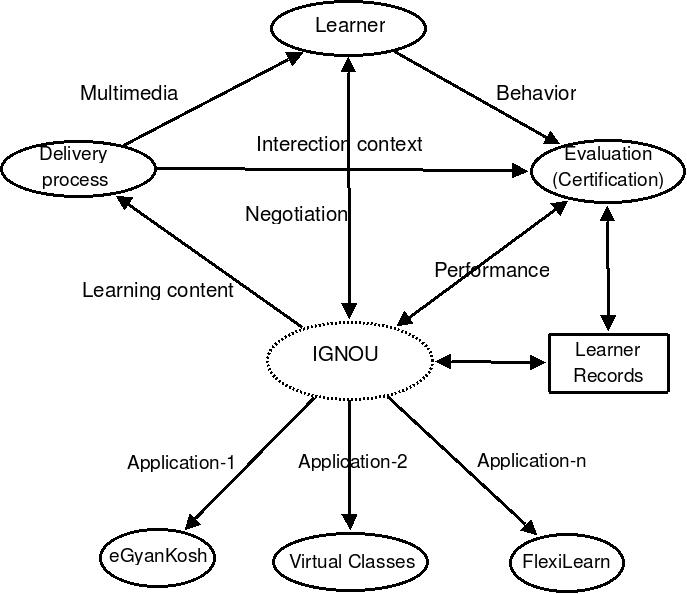
\includegraphics[scale=.5]{flexi1.jpeg}
 % flexi1.jpeg: 687x594 pixel, 72dpi, 24.24x20.95 cm, bb=0 0 687 594
 \caption{FlexiLearn Distributed System Architecture}
\end{figure}
\begin{figure}[htb]
 \centering
 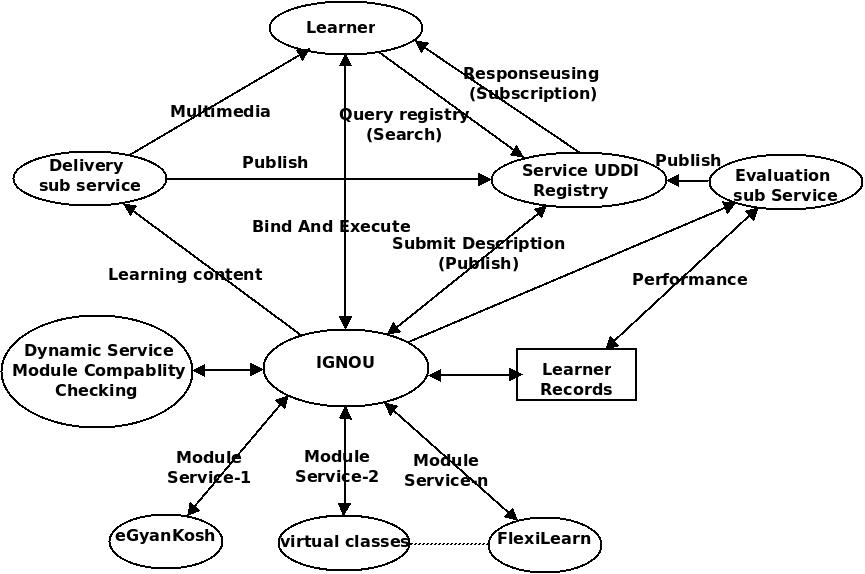
\includegraphics[scale=.5]{ignousoa2.jpeg}
 % flexisoajournal.jpeg: 898x583 pixel, 72dpi, 31.68x20.57 cm, bb=0 0 898 583
 \caption{FexiLearn system in IEEE LTSA mapped in SOA}
\end{figure}

\section{Limitation of present Flexilearn system}
\blindtext
\section{Comparision of IGNOU online services in terms of composition of services}
\blindtext
\section{Security Capacity in the Proposed Model in SOA}
\blindtext
\subsection{Approach To Protecting Services}
\blindtext

\subsubsection{Protect services from the outside at deployment time by using WSM (web service manager) solutions}
\blindtext
\subsubsection{Protect services from the inside by building security into software development process}
Devloper of e-Learning services must validate the input usually in XML document format. Various types of attacks are, buffer overflow, SQL injection, XML injection,
and XPath exploits. Static analytical tools are used for identifying such vulnerabilities.
\subsubsection{Simulation of known attack patterns and fixing vulnerabilities}
Dynamic analysis tools are used during the query and analysis (QA) process to
test, verify and validate the actual deployment. Stress-testing of SOA applications
calls for designing different attack patterns. Vulnerabilities may be uncovered and
resolved before deployment. This may be considered under preventive security
maintenance.
\subsubsection{Monitoring WSM solutions}
\blindtext
\subsection{Protecting Services from the Outside}
\blindtext


\flushbottom

\flushbottom
\blindtext\chapter{Composition of e-Learning Web Services in SOA}
\blindtext  \cite{com, com2}.
\section{e-Learning web Services}
\blindtext
\begin{itemize}
 \item Registration Service
\item Computer Programming Lectures service (Textual Narratives)
\item  Computer Programming Lectures service (Multimedia Narratives)
\item Online Examination Service
\end{itemize}

\begin{table}
 \begin{center}
 \caption{2nd Sample Table}
 \begin{tabular}{|c|c|}
 \hline
 B.Tech & CSE\\
 \hline
 M.Tech & ECE\\
 \hline
 Ph.D & EIE\\
 \hline 
 \end{tabular}
 \end{center}
\end{table}

\subsection{Registration Service}
Registration Service is the service to check whether a user, going to utilize the service is authorized user or not. If user is already registered
then he/she is allowed to avail the services otherwise, he/she is provided with 'register service' where he/she has to register first to access the services. This registration service 
has two functions 'Login' and 'Register'. Login method is to get into the system after successfull authentication such as login ID 
and 'Register method' is to register a user if he/she is not already the member of e-Learning system. (Figure.8)   

\begin{table}
 \begin{center}
 \caption{3rd Sample Table}
 \begin{tabular}{|c|c|}
 \hline
 B.Tech & CSE\\
 \hline
 M.Tech & ECE\\
 \hline
 Ph.D & EIE\\
 \hline 
 \end{tabular}
 \end{center}
\end{table}

%\begin{figure}[h!]
 %\centering
 %\includegraphics[width=16cm,height=13cm]{Register_Service_function_invoke.jpg}
 % Register_Service_function_invoke.jpg: 1024x768 pixel, 96dpi, 27.09x20.32 cm, bb=
%\caption{Registeration Service Invocation}
%\end{figure}
%\end{comments}

\subsection{Computer Programming Service (Textual Narratives)}
Computer Programming Lectures service (textual nrration) is service which provides the facility of downloading lectures in doc and 
pdf form. This service can only be accessed if the user is authorized by the system (Figure.9). 

\begin{table}
 \begin{center}
 \caption{4th Sample Table}
 \begin{tabular}{|c|c|}
 \hline
 B.Tech & CSE\\
 \hline
 M.Tech & ECE\\
 \hline
 Ph.D & EIE\\
 \hline 
 \end{tabular}
 \end{center}
\end{table} 
%\begin{figure}[h!]
% \centering
% \includegraphics[width=16cm,height=13cm]{CP_Service_main.JPG}
 %% CP_Service_main.JPG: 1024x768 pixel, 96dpi, 27.09x20.32 cm, bb=
 %\caption{Computer Programming Service}
%\end{figure}


\subsection{Computer Programming Service (Multimedia Narratives)}
Computer Programming Lectures service (Multimedia Narratives) is the service which provides the facility of downloading audio/video lectures
 This service can only be accessed if the user is authorized by the system and the client system is having the authorized player of the files. 
 
 \begin{table}
 \begin{center}
 \caption{5th Sample Table}
 \begin{tabular}{|c|c|}
 \hline
 B.Tech & CSE\\
 \hline
 M.Tech & ECE\\
 \hline
 Ph.D & EIE\\
 \hline 
 \end{tabular}
 \end{center}
\end{table} 
\subsection{Online Examination Service}
Online examination is examination system in which user can give the exam at his own pace limited by the system.
Online examination service is basis of the online certification of courses. On-line examination service is used to check the ability 
of a user in computer programming. As soon as user gets authorized he/she can access this service and can attempt questions online through the examination
 process. After the successful submission of examination answering, the user will get the result immediately (Figure. 10). 
 
 \begin{table}
 \begin{center}
 \caption{6th Sample Table}
 \begin{tabular}{|c|c|}
 \hline
 B.Tech & CSE\\
 \hline
 M.Tech & ECE\\
 \hline
 Ph.D & EIE\\
 \hline 
 \end{tabular}
 \end{center}
\end{table} 
%\begin{figure}[h!]
% \centering
% \includegraphics[width=16cm,height=13cm]{Exam_Service_main.jpg}
 % Exam_Service_main.jpg: 1024x768 pixel, 96dpi, 27.09x20.32 cm, bb=0 0 768 576
 %\caption{Online Exam Service}
%\end{figure}



\section{e-Learning Web Services: Publish and Subscription Methodology}
e-Learning system composed of number of services, some of them are primary web services and some are secondary as per need. Primary 
service are used for the coordination of other services as UDDI service and  compatibility checking service. Secondary services 
include fully functioned stand alone services as registration service, online examination service, etc.

\begin{table}
 \begin{center}
 \caption{7th Sample Table}
 \begin{tabular}{|c|c|}
 \hline
 B.Tech & CSE\\
 \hline
 M.Tech & ECE\\
 \hline
 Ph.D & EIE\\
 \hline 
 \end{tabular}
 \end{center}
\end{table}
\subsection{Publishing e-Learning Web Services into UDDI}
The e-Learning system, for local UDDI, is prepared and presented through the web portal (Figure 11) .UDDI service in Microsoft Web Server 2008 is configured.  Registration service, Computer 
Programming Service (Texual Narratives), Computer Programming Service (Multimedia narratives) and online examination services are published on different
systems and registered with service provider's name to UDDI by publish service of UDDI \cite{support, uddi, service}. UDDI Service 
requires Provider's name and the service’s WSDL file for it’s publication in UDDI registry. The process is shown in figure.11; 12; 13.

\begin{table}
 \begin{center}
 \caption{8th Sample Table}
 \begin{tabular}{|c|c|}
 \hline
 B.Tech & CSE\\
 \hline
 M.Tech & ECE\\
 \hline
 Ph.D & EIE\\
 \hline 
 \end{tabular}
 \end{center}
\end{table}

% \begin{figure}[h!]
% \centering
% \includegraphics[width=16cm,height=13cm]{uddi_home_interface.jpg}
%\caption{UDDI home Interface}
 % uddi_home_interface.jpg: 1024x768 pixel, 96dpi, 27.09x20.32 cm, bb=0 0 768 576
%\end{figure}
%\begin{figure}[h!]
% \centering
% \includegraphics[width=16cm,height=13cm]{provider_interface.jpg}
%\caption{UDDI Provider Interface}
 % provider_interface.jpg: 1022x544 pixel, 96dpi, 27.04x14.39 cm, bb=0 0 767 408
%\end{figure}
%\begin{figure}[h!]
% \centering
 %\includegraphics[width=16cm,height=13cm]{uddi_add_service.jpg}
 % uddi_add_service.jpg: 1019x683 pixel, 96dpi, 26.96x18.07 cm, bb=0 0 764 512
 %\caption{UDDI Add Service Interface}
%\end{figure}
\begin{itemize}
 
\item On the configured UDDI Services home page 'Publish' button is clicked. The configured UDDI open the page 'My UDDI'.
\item On the 'My UDDI' page, the Providers tab is clicked and a number of options is shown through the menu.
\item On the Providers tab, 'Add Provider' is chosen to be clicked. The 'My UDDI' (New Provider Name) page appears in the browser for 
providing option to add new providers name. 
\item On the 'My UDDI' (New Provider Name) page, the Edit button 'under actions' is chosen to be clicked. The name is required to be edit. The 'Name' text button
appears.
\item In the 'Name' textbox,  New WebService is typed, and then Update button is clicked. The 'My UDDI' (NewWebService) page appears again in the browser with all the added information.
\item 'My UDDI' (NewWebService) page provides the services, that is required to be checked then Add Service is another option that is avilable
in this option. It is clicked. A number of options are again available.
\item Under Actions, option Edit is selected to be clicked, the textbox of 'Name' is filled with service 1. The next step is to update 
the information by clicking Update.
\item  On the 'My UDDI' New Service 1 page, Bindings tab appears with a number of options.
\item Add Binding tab is activated by clicking.
\item Again the 'My UDDI' NewWebService Service1 http://'' page, Edit button is chosen to be clicked. The Access Point textbox appears.
\item In the Access Point textbox, the URL of the services composed is typed. Update button is clicked for required updation 
$http://computer\_name/Service1.asmx$
In the URL, computer\_name is replaced with the name of the server that hosts the Web service. $``http://localhost''$ in the URL should not be used..
\item On the UDDI Services page, the 'Instance Info' tab is clicked.
\item Again, on the Instance Info tab, Add Instance Information is checked out. 
\end{itemize}

\begin{table}
 \begin{center}
 \caption{9th Sample Table}
 \begin{tabular}{|c|c|}
 \hline
 B.Tech & CSE\\
 \hline
 M.Tech & ECE\\
 \hline
 Ph.D & EIE\\
 \hline 
 \end{tabular}
 \end{center}
\end{table}

The client system searches the required services and their location, other details of services which are required to use those 
services are obtained. These services required to be composed, are available so that a learner or visitor to our 
e-Learning system can get the access of these services in a user friendly manner. 
\subsection{Searching e-Learning Web Services in UDDI}
Web services can be searched in UDDI by using the keywords. 'Search' function of UDDI returns the service provider name, Service location 
with other details, through it’s WSDL detail (Figure. 14).
\begin{figure}[h!]
 \centering
 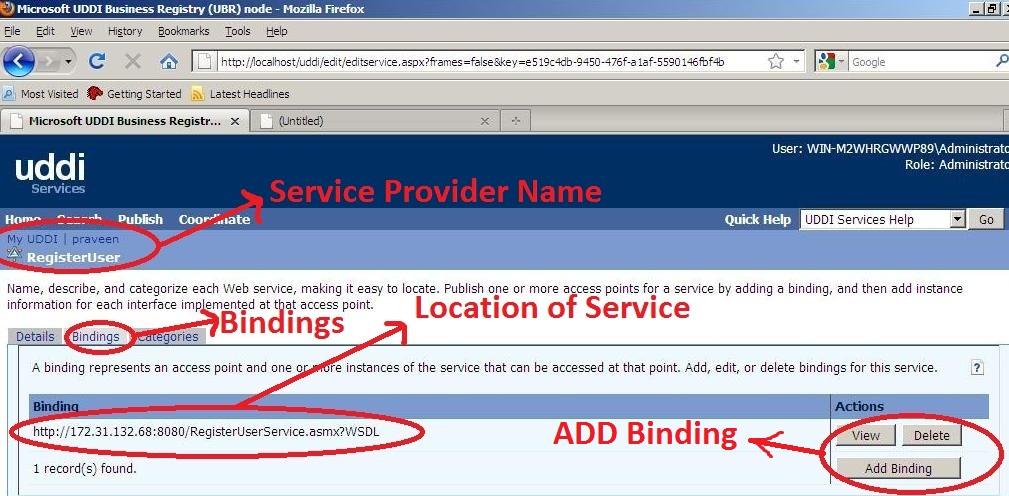
\includegraphics[width=16cm,height=13cm]{uddi_service_binding_interface.jpg}
 % uddi_service_binding_interface.jpg: 1009x496 pixel, 96dpi, 26.70x13.12 cm, bb=0 0 757 372
 \caption{UDDI Service Binding Interface}
\end{figure}

\begin{table}
 \begin{center}
 \caption{10th Sample Table}
 \begin{tabular}{|c|c|}
 \hline
 B.Tech & CSE\\
 \hline
 M.Tech & ECE\\
 \hline
 Ph.D & EIE\\
 \hline 
 \end{tabular}
 \end{center}
\end{table}
\section{e-Learning  Web  Services: Composition Technique}
To provide learning facility to the user we considered three types of e-Learning services
\begin{itemize}
\item Computer programming Service (Textual Narratives)
\item Computer programming Service (Multimedia Narratives)
\item Online Examination Service

\end{itemize}

\begin{table}
 \begin{center}
 \caption{11th Sample Table}
 \begin{tabular}{|c|c|}
 \hline
 B.Tech & CSE\\
 \hline
 M.Tech & ECE\\
 \hline
 Ph.D & EIE\\
 \hline 
 \end{tabular}
 \end{center}
\end{table}
\begin{figure}[h!]
 \centering
 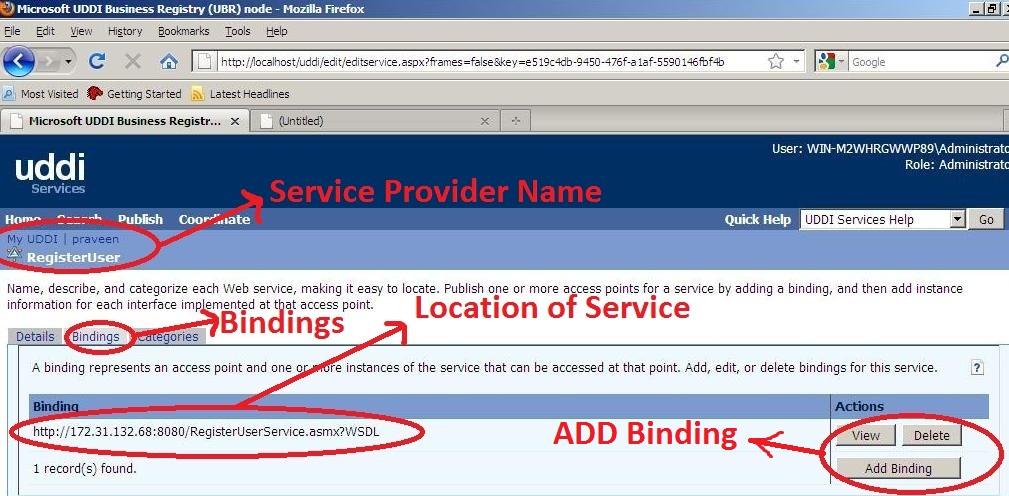
\includegraphics[width=16cm,height=13cm]{uddi_service_binding_interface.jpg}
 % uddi_service_binding_interface.jpg: 1009x496 pixel, 96dpi, 26.70x13.12 cm, bb=0 0 757 372
 \caption{UDDI Service Binding Interface}
\end{figure}
Each of these services is stand alone and totally independent from others. Besides these services, there are other services 
like registration service, this is also stand alone and independent service registration service. Registration service can be composed to every of the service mentioned above. 


\begin{table}
 \begin{center}
 \caption{12th Sample Table}
 \begin{tabular}{|c|c|}
 \hline
 B.Tech & CSE\\
 \hline
 M.Tech & ECE\\
 \hline
 Ph.D & EIE\\
 \hline 
 \end{tabular}
 \end{center}
\end{table}
\subsubsection{Composition of Computer Programming Service (Textual Narratives) with Registration Service}
\blindtext
\begin{figure}[h!]
 \centering
 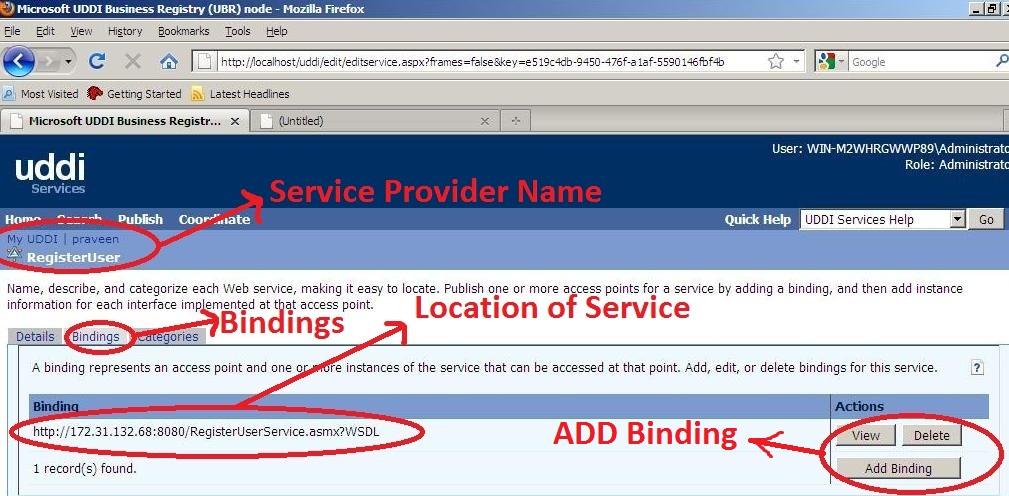
\includegraphics[width=16cm,height=13cm]{uddi_service_binding_interface.jpg}
 % uddi_service_binding_interface.jpg: 1009x496 pixel, 96dpi, 26.70x13.12 cm, bb=0 0 757 372
 \caption{UDDI Service Binding Interface}
\end{figure}

\begin{table}
 \begin{center}
 \caption{13th Sample Table}
 \begin{tabular}{|c|c|}
 \hline
 B.Tech & CSE\\
 \hline
 M.Tech & ECE\\
 \hline
 Ph.D & EIE\\
 \hline 
 \end{tabular}
 \end{center}
\end{table}
\subsubsection{Computer Programming Service (Multimedia Narratives) Composition with Registration Service}
\Blindtext
\begin{figure}[h!]
 \centering
 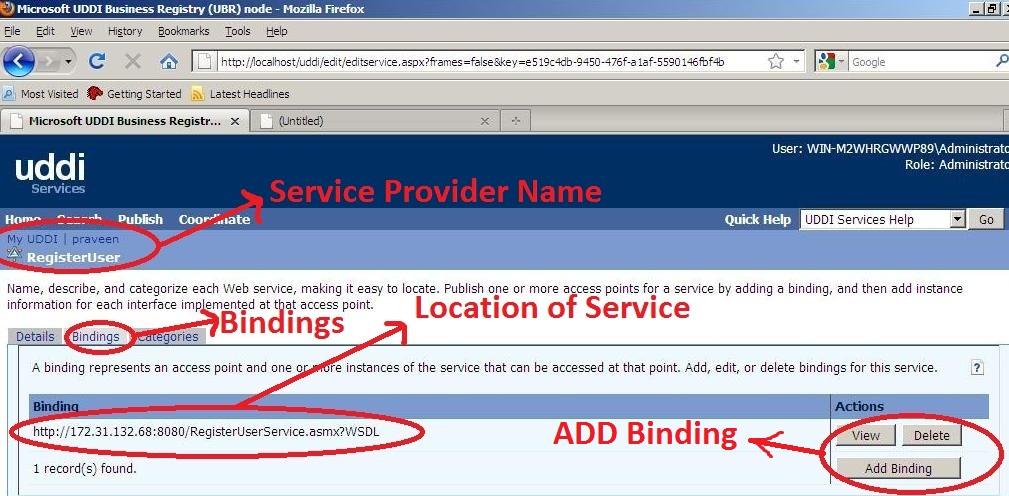
\includegraphics[width=16cm,height=13cm]{uddi_service_binding_interface.jpg}
 % uddi_service_binding_interface.jpg: 1009x496 pixel, 96dpi, 26.70x13.12 cm, bb=0 0 757 372
 \caption{UDDI Service Binding Interface}
\end{figure}

\begin{table}
 \begin{center}
 \caption{14th Sample Table}
 \begin{tabular}{|c|c|}
 \hline
 B.Tech & CSE\\
 \hline
 M.Tech & ECE\\
 \hline
 Ph.D & EIE\\
 \hline 
 \end{tabular}
 \end{center}
\end{table}
\subsubsection{Online Examination Service  Composition with Registration Service}
\Blindtext
\begin{figure}[h!]
 \centering
 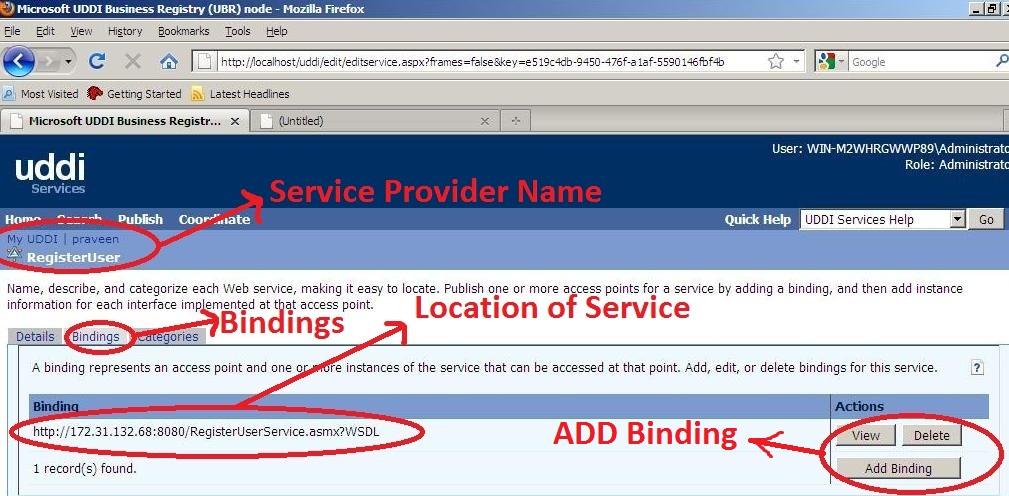
\includegraphics[width=16cm,height=13cm]{uddi_service_binding_interface.jpg}
 % uddi_service_binding_interface.jpg: 1009x496 pixel, 96dpi, 26.70x13.12 cm, bb=0 0 757 372
 \caption{UDDI Service Binding Interface}
\end{figure}

\begin{table}
 \begin{center}
 \caption{15th Sample Table}
 \begin{tabular}{|c|c|}
 \hline
 B.Tech & CSE\\
 \hline
 M.Tech & ECE\\
 \hline
 Ph.D & EIE\\
 \hline 
 \end{tabular}
 \end{center}
\end{table}
\subsection{e-Learning Web Service Composition Algorithm}
Web services composition synchronization is achieved from services compatability and their on-the-fly binding from the option like'Add References'. When Registration service gets composed with computer programming service and online examination service the method makes application of the value of service for storing in a variable. 
After the successful completion of registration service the value stored in the variable is checked.     

\begin{algorithm*}[!htb]
\caption{Service Composition Method: A Sample}
\begin{code}
\uln \>\ubegin\\
\uln \>\>  $Get\ service\ choice\ from\ user$\\
\uln \>\>\> $Save\ choice\ into\ a\ variable\ 'var'$ \\
\uln \>\> $Call \ Login \ Service \ with\ a \ argument\ of \ saved \ variable\ (var)$\\
\uln \>\>\> $Do\ Login\ (validation)$\\
\uln \>\>\>\uif $user\ is\ valid$) \uthen\\
\uln \>\>\>\> $check\ variable$\ (var)\\
\uln \>\>\>\> $call\ service\ which\ refer\ to\ (var) $)\\
\uln \>\>\>\> $Get\ the\ result\ of\ service  $\\
\uln \>\>\>\> $Return\ result$\\
\uln \>\>\>\uelse  $Return\ error\ to\ caller\ of\ Login\ Function$  \\
\uln \>\uend\\ 
\end{code}
\label{alg:dfs}
\end{algorithm*}


\section{e-Learning Web Portal: e-Learning Web Services and their Composition}
The e-Learning portal under consideration provides three application that make use of the programming  services to the end user computer programming service in doc, pdf document downloads,
in audio/video file downloads and online examination to the end user. These functions are simple application through GUI in the stand alone
mode in a client service architecture. However, the access and composition of these services for different application from different nodes
at different logical locations calls for capacity building in distributed system architecture and compatability governance in service oriented architecture. 
 \begin{figure}[h!]
 \centering
 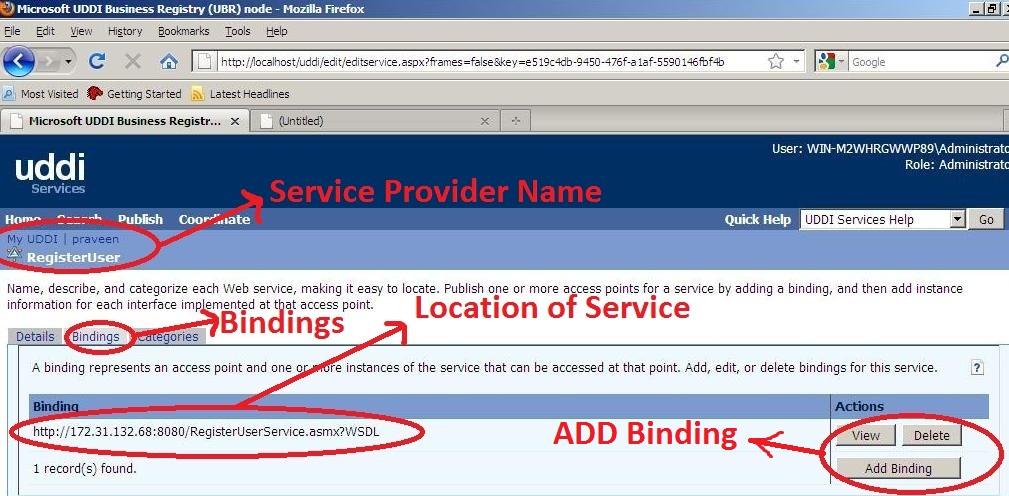
\includegraphics[width=16cm,height=13cm]{uddi_service_binding_interface.jpg}
 % uddi_service_binding_interface.jpg: 1009x496 pixel, 96dpi, 26.70x13.12 cm, bb=0 0 757 372
 \caption{UDDI Service Binding Interface}
\end{figure} 
\subsection{Home page of the e-Learning web portals}
Home page shows the sample services provided by e-Learning web portal. The services may be identified and accessed by the identity of service name. The functionality and implementation  of services are hidden from the user and provides only output by interactive GUI to the user. Home Page shows links to all services availlable
in the designed e-Learning web portal. By clicking these link user can access the complete functioality of composite services which are unknown to him/her earlier.\par
Home Page contains three links for each services (Computer Programming Service, Audio/video service and Online Examination service).
The user can select any one of the service and can get composed service with Registration service (Figure. 17) with one of the available services.
\begin{figure}[h!]
 \centering
 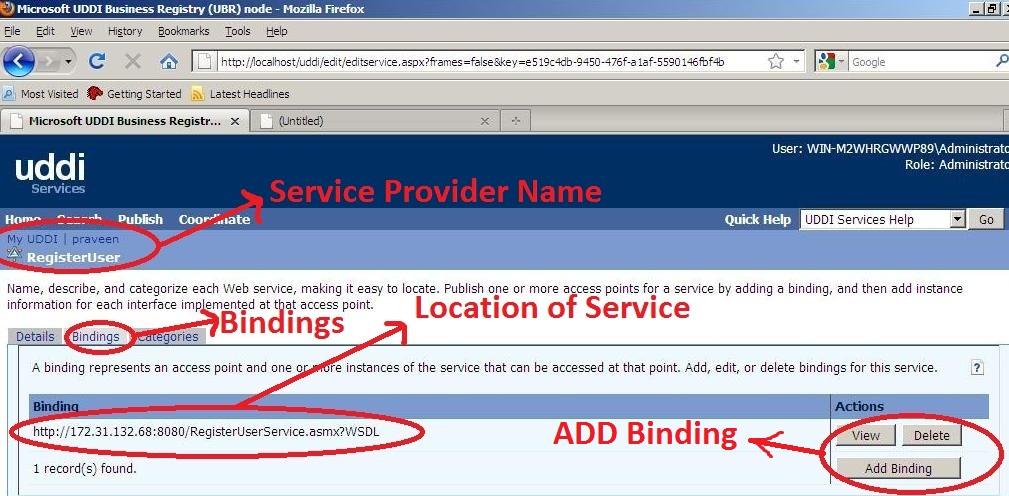
\includegraphics[width=16cm,height=13cm]{uddi_service_binding_interface.jpg}
 % uddi_service_binding_interface.jpg: 1009x496 pixel, 96dpi, 26.70x13.12 cm, bb=0 0 757 372
 \caption{UDDI Service Binding Interface}
\end{figure} 
%\begin{figure}[h!]
% \centering
% \includegraphics[width=16cm,height=13cm]{Application_home.jpg}
 % Application_home.jpg: 1024x768 pixel, 96dpi, 27.09x20.32 cm, bb=0 0 768 576
% \caption{Home page of the e-Learning web portal}
%\end{figure}
\subsection{Login page of the e-Learning Web Portal}
When user click on any of the service links in the Home page, Login Page is presented on the monitor. If the user is not registered then he/she has to get registered first. for that he/she has to 
click on the register link (Figure.18) as shown.
\begin{figure}[h!]
 \centering
 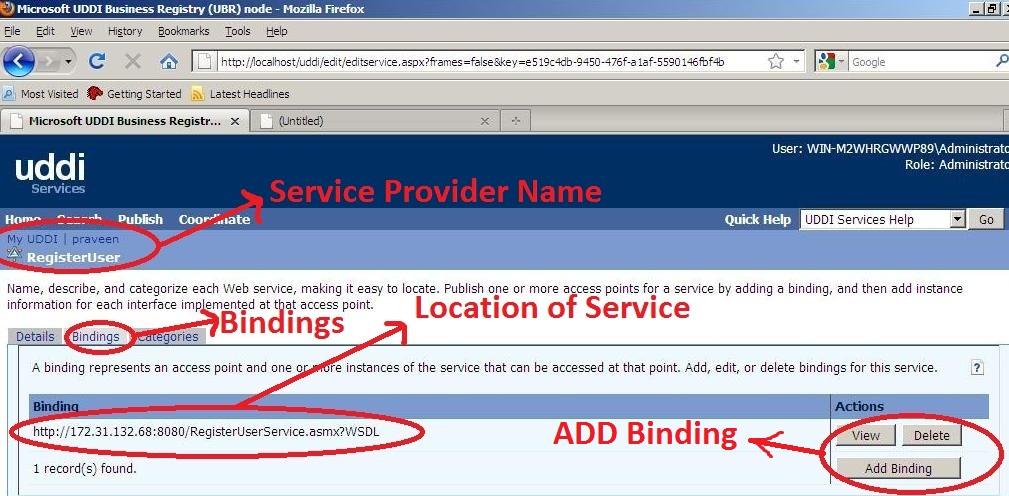
\includegraphics[width=16cm,height=13cm]{uddi_service_binding_interface.jpg}
 % uddi_service_binding_interface.jpg: 1009x496 pixel, 96dpi, 26.70x13.12 cm, bb=0 0 757 372
 \caption{UDDI Service Binding Interface}
\end{figure}
%\begin{figure}[h!]
% \centering
% \includegraphics[width=16cm,height=13cm]{Application_login.jpg}
 % Application_login.jpg: 1024x768 pixel, 96dpi, 27.09x20.32 cm, bb=0 0 768 576
 %\caption{Login Page}
%\end{figure}
\subsection{Registration Page of the e-Learning Web Portal}
If user is already registered then he can access services through login process. If the user is not registered  then he/she has to register first by
filling the Registarion page. He/She has to fill the required fields and submit for registration. 
The user is allowed to access other services which are composed with 
Registration service. Login service itself is automatically invoked when the user chooses to click on any service link (Figure. 19).
\begin{figure}[h!]
 \centering
 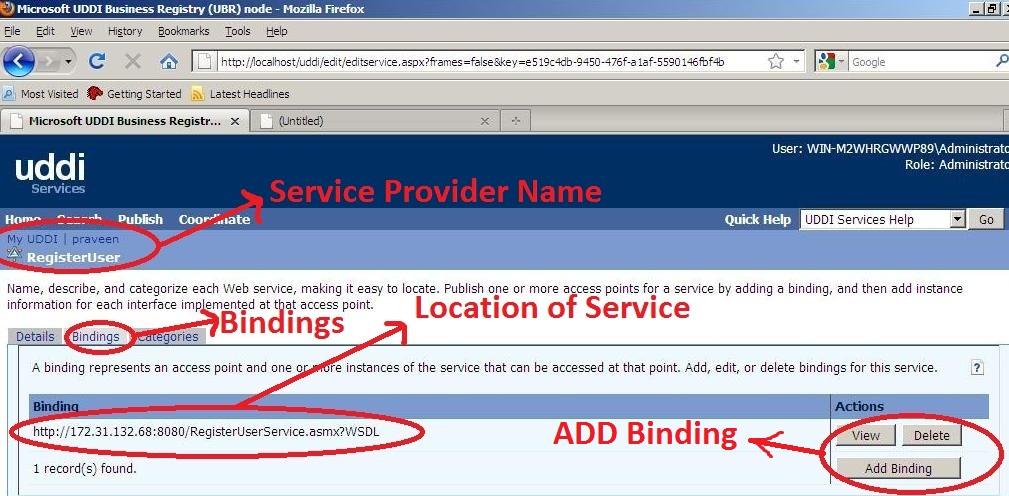
\includegraphics[width=16cm,height=13cm]{uddi_service_binding_interface.jpg}
 % uddi_service_binding_interface.jpg: 1009x496 pixel, 96dpi, 26.70x13.12 cm, bb=0 0 757 372
 \caption{UDDI Service Binding Interface}
\end{figure}
%\begin{figure}[h!]
% \centering
 %\includegraphics[width=16cm,height=13cm]{Application_register.jpg}
 % Application_register.jpg: 1024x768 pixel, 96dpi, 27.09x20.32 cm, bb=0 0 768 576
 %\caption{Register Page}
%\end{figure}
\subsection{Programming Service page the of e-Learning Web Portal}
The e-Learning link on the Home Page provides the Registration service for user authentication. If the user is authorized then Programming Service Page offers the downloading-services from where user can download the lectures in doc or pdf format.
Programming Service (textual/Multimedia narratives) is also similar in capacity to Programming Service for the lectures in doc or pdf format (Figure. 20) 
\begin{figure}[h!]
 \centering
 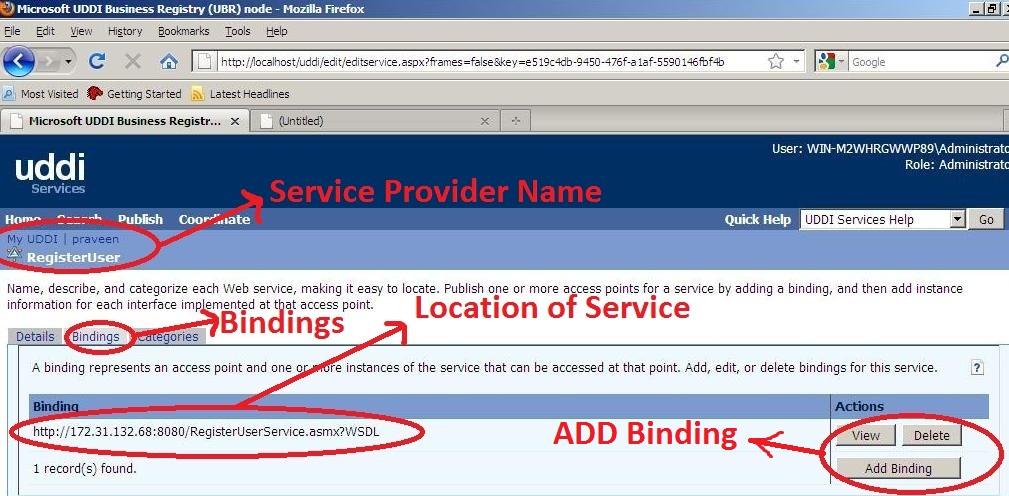
\includegraphics[width=16cm,height=13cm]{uddi_service_binding_interface.jpg}
 % uddi_service_binding_interface.jpg: 1009x496 pixel, 96dpi, 26.70x13.12 cm, bb=0 0 757 372
 \caption{UDDI Service Binding Interface}
\end{figure}

\subsection{Online Examination Page of e-Learning web portal}
Online Exam page gets opened from the link on Home page. The service first invokes Login page on the monitor. The user is already
registered then the user can avail the examination service. Otherwise the user has to register himself/herself first (Figure.21).
\begin{figure}[h!]
 \centering
 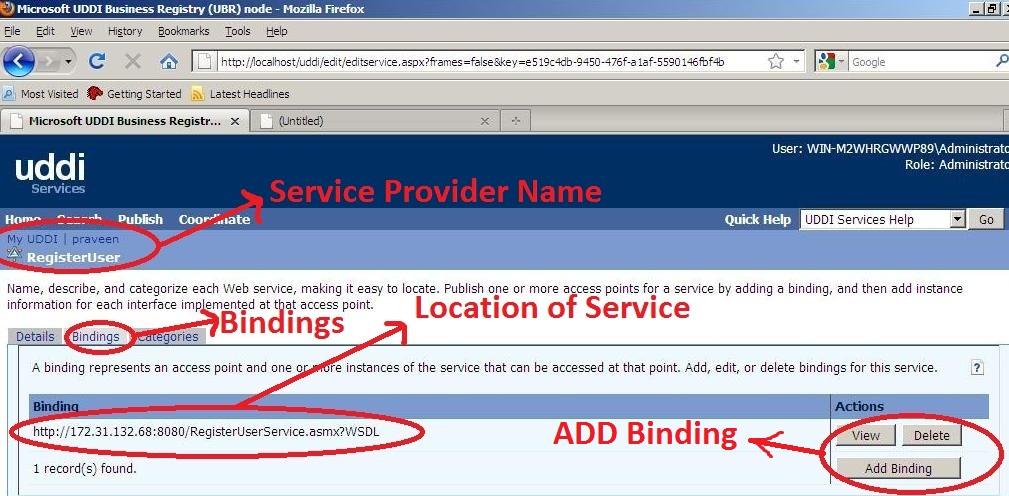
\includegraphics[width=16cm,height=13cm]{uddi_service_binding_interface.jpg}
 % uddi_service_binding_interface.jpg: 1009x496 pixel, 96dpi, 26.70x13.12 cm, bb=0 0 757 372
 \caption{UDDI Service Binding Interface}
\end{figure}
\flushbottom

\flushbottom
\chapter{Conclusion \& Future Direction of Work}
\section{Conclusion}
  \blindtext
 
\section{Future Direction of work} In \blindtext part OWL.\\

The prospect of research of research orientation in this field  encourage one to reactive more in composite web services in SOA.


\flushbottom

\begin{thebibliography}{11}
%\itemsep0em
\bibitem{cc}
Eric Gamess and Imad Mahgoub.
\newblock A Novel VANET-Based Approach to Determine the Position of the Last Vehicle Waiting at a Traffic Light.
\newblock In {\em The 2011 International Conference on Wireless Networks (ICWN ’11)}, July 2011.

\bibitem{lan}
E. Bas, M. Tekalp, and F. Salman.
\newblock Automatic Vehicle Counting from Video for Traffic Flow Analysis.
\newblock In {\em 2007 IEEE Intelligent Vehicles Symposium}, Istanbul, Turkey. June 2007.

\bibitem{com}
P. Daigavane and P. Bajaj.
\newblock Real Time Vehicle Detection and Counting Method for Unsupervised Traffic Video on Highways.
\newblock In {\em International Journal of Computer Science and Network Security}, Vol. 10, No. 8. August 2010.

\bibitem{car}
C. Pornpanomchai, T. Liamsanguan, and V. Vannakosit.
\newblock Vehicle Detection and Counting from a Video Frame.
\newblock In {\em International Conference on Wavelet Analysis and Pattern Recognition (ICWAPR ’08)}, Hong Kong. September 2008.
 
\bibitem{com2}
M. Lei, D. Lefloch, P. Gouton, and K. Madani.
\newblock A Video-Based Real-Time Vehicle Counting System Using Adaptive Background Method.
\newblock {\em The Fourth International Conference on Signal-Image Technology and Internet Based Systems (SITIS’08)}, Bali, Indonesia. December 2008.

\bibitem{ltsa}
M. Litzenberger, B. Kohn, G. Gritsch, N. Donath, C. Posch, N.A. Belbachir, and H. Garn. 
\newblock Vehicle Counting with an Embedded Traffic Data System using an Optical Transient Sensor. 
\newblock In {\em The 10th International IEEE Conference on Intelligent Transportation Systems (ITSC ’07)}, Seattle, WA, USA. September 2007.

\bibitem{gill}
Caballero-Gil, P. 
\newblock Security Issues in Vehicular Ad Hoc Networks.
\newblock University of La Laguna, Spain.

\bibitem{sp}
Seuwou, P., Patel, D., Protheroe, D., Ubakanma, G.
\newblock Effective security as an ill-defined problem in vehicular ad hoc networks (VANETs). 
\newblock In {\em Road Transport Information and Control (RTIC 2012)}, IET and ITS Conference on (pp. 1-6). IET.

\bibitem{omnetpp}
Andr$\acute{a}$s Varga and OpenSim Ltd.
\newblock OMNeT++ User Manual Version 4.2.2

\end{thebibliography}

%\begin{comment}
\appendix 
\renewcommand{\thechapter}{\Roman{chapter}}
\chapter{Publications Related to Report Work}
\begin{enumerate}	
 \item  Kumar, Prveen., Samaddar, Shefalika Ghosh., Samaddar, Arun B. \& Misra, Arun K.,
 (2010); \textbf{Extending IEEE LTSA e­learning Framework in Secured SOA Environment}, 
  The 2nd IEEE International Conference on Education Technology and Computer (ICETC 2010),
 IEEE Education Society (ISBN: 978-1-4244-6368-8), Shanghai China, June 22-­24, 2010. 
\textbf{(Accepted)}
\item   Kumar, Prveen., Samaddar, Shefalika Ghosh., Samaddar, Arun B. \& Misra,
 Arun K.(2010); \textbf{Extending IEEE LTSA e­learning Framework in Secured SOA Environment}, 
  IEEE Transaction on Leatning Technology. \textbf{(Under Peer Review)}
\end{enumerate}
%\end{comment}

\pagestyle{fancy}
\fancyhead[RO,RE]{Biographical Sketch}
\chapter{Biographical Sketch}
\begin{center}
{\textbf{\LARGE First Student's Name}}\end{center} %\hrule
\begin{center}
Madhya Banamalipur, West Side of Central Jail, Agartala  PIN-799001,  E-Mail: abc@gmail.com,  Contact. No. +91-1234567890 \\
 \end{center}
 \begin{itemize}
\item Pursuing B.Tech. in Computer Sc. \& Engg. branch from N.I.T,Agartala with CPI of 8.34/10/00.
\item Intermediate from N.S.Vidyaniketan,Agartala under (T.B.S.E), Tripura with 58\% in 1996.
\item High School from N.S.Vidyaniketan,Agartala under (T.B.S.E), Tripura with 60.66 \% in 1994.
\end{itemize}

\begin{center}
{\textbf{\LARGE Second Student's Name}}\end{center} %\hrule
\begin{center}
Madhya Banamalipur, West Side of Central Jail, Agartala  PIN-799001,  E-Mail: abc@gmail.com,  Contact. No. +91-1234567890 \\
 \end{center}
 \begin{itemize}
\item Pursuing B.Tech. in Computer Sc. \& Engg. branch from N.I.T,Agartala with CPI of 8.34/10/00.
\item Intermediate from N.S.Vidyaniketan,Agartala under (T.B.S.E), Tripura with 58\% in 1996.
\item High School from N.S.Vidyaniketan,Agartala under (T.B.S.E), Tripura with 60.66 \% in 1994.
\end{itemize}

\begin{center}
{\textbf{\LARGE Third Student's Name}}\end{center} %\hrule
\begin{center}
Madhya Banamalipur, West Side of Central Jail, Agartala  PIN-799001,  E-Mail: abc@gmail.com,  Contact. No. +91-1234567890 \\
 \end{center}
 \begin{itemize}
\item Pursuing B.Tech. in Computer Sc. \& Engg. branch from N.I.T,Agartala with CPI of 8.34/10/00.
\item Intermediate from N.S.Vidyaniketan,Agartala under (T.B.S.E), Tripura with 58\% in 1996.
\item High School from N.S.Vidyaniketan,Agartala under (T.B.S.E), Tripura with 60.66 \% in 1994.
\end{itemize}

\begin{center}
{\textbf{\LARGE Fourth Student's Name}}\end{center} %\hrule
\begin{center}
Madhya Banamalipur, West Side of Central Jail, Agartala  PIN-799001,  E-Mail: abc@gmail.com,  Contact. No. +91-1234567890 \\
 \end{center}
 \begin{itemize}
\item Pursuing B.Tech. in Computer Sc. \& Engg. branch from N.I.T,Agartala with CPI of 8.34/10/00.
\item Intermediate from N.S.Vidyaniketan,Agartala under (T.B.S.E), Tripura with 58\% in 1996.
\item High School from N.S.Vidyaniketan,Agartala under (T.B.S.E), Tripura with 60.66 \% in 1994.
\end{itemize}

\end{document}